\RequirePackage{luatex85}
\documentclass{standalone}

\usepackage{fontspec, unicode-math}
\setsansfont[Scale=MatchLowercase]{TeX Gyre Heros}
\setmathfont{TeX Gyre Termes Math}

\usepackage{pgfplots}
\pgfplotsset{compat=1.14}

\tikzset{
  every picture/.style={font={\sffamily\normalsize}, >=stealth},
  every pin edge/.style={black}}

\begin{document}

  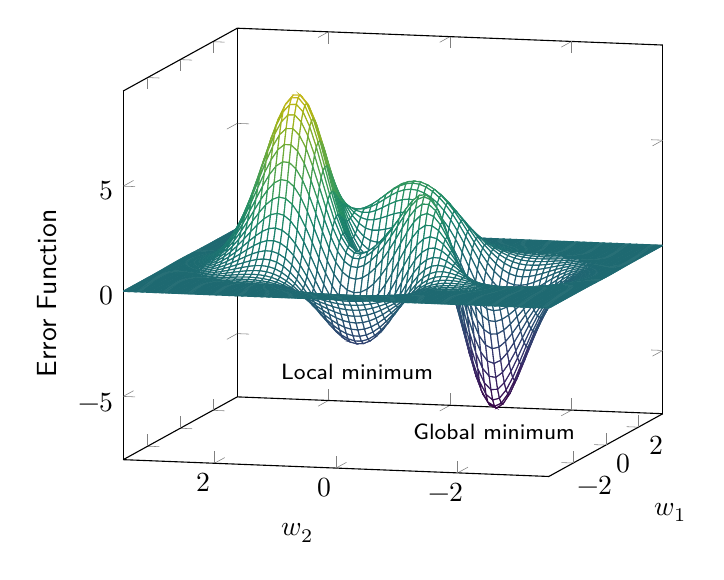
\begin{tikzpicture}[%
    dots/.style={circle, fill, inner sep=2pt},
    every label/.append style={font=\sffamily\footnotesize}]

    \begin{axis}[colormap/viridis,
      xlabel = {$w_{1}$},
      ylabel = {$w_{2}$},
      zlabel = {Error Function},
      view = {-75}{10},
      declare function = {
        f(\x,\y) = 3*(1-\x)^2*exp(-\x^2-(\y+1)^2)-10*(\x/5-\x^3-\y^5)*exp(-\x^2-\y^2)-1/3*exp(-(\x+1)^2-\y^2);}]

      \addplot3[surf, fill=white, domain=-3.5:3.5, samples=65]{f(x,y)};

      \node[label={270:{Local minimum}}] at (axis cs:-0.82020, 0.3725, -3.3) {};
      \node[label={270:{Global minimum}}] at (axis cs:0.05, -1.65, -6.28390) {};
    \end{axis}
  \end{tikzpicture}

\end{document}
